\section{Algorithm}
\label{s:algorithm}

We use the algorithm proposed by Orlovich and Rugina~\cite{rugina}. It is a 
backward Dataflow analysis, validating a statement's safety by searching for 
contradictions. It releases a detection probe for each suspicious statement 
that might lead to a loss of the last reference to a heap cell, assuming that 
a memory leak happens. A backward Dataflow analysis is immediately started from
that program point to check whether contradiction exist on all possible 
branches, which then proves that the probe statement is safe. If the Dataflow analysis 
reaches a $\top$ or the program entry is reached, the analysis reports a 
potential memory leak.


\subsection{Core Imperative Language}
\label{ss:semantics}

In this section we describe the core imperative language 
used by the algorithm, which helps better understand the later sections.

\paragraph{Syntax} 
\begin{align*}
  Statements s\in St s:: &= *e_0\gets e_1\ |\ *e\gets malloc\ |\ free(e)\ |\ \\
                         &     cond(e_0\equiv e_1)\ |\ return e\ |\ enter \\
  Expressions e\in E e:: &= n\ |\ a\ |\ *e\ |\ e.f\ |\ e_0 \oplus e_1 
\end{align*}

where, 
\begin{align*}
  n\in \mathbb{Z} &\text{  ranges over numeric constants $(NULL=0)$}, \\
  a\in \mathbb{A} &\text{  over symbolic addresses,} \\
  f\in \mathbb{F} &\text{  over structure fields,} \\
           \oplus &\text{  over arithmetic operators,} \\
           \equiv &\text{  over the comparison operators $=$ and $\ne$.}
\end{align*}


\paragraph{Mem(e) Function} 

The set $Mem(e)$ denotes the subexpressions of $e$ that represent memory 
locations. This set is defined recursively as follows:

\begin{align*}
  Mem(n) &= Mem(a)=\emptyset \\
Mem(e.f) &= Mem(e) \\
 Mem(*e) &={*e}\cup Mem(e) \\
Mem(e_0 \oplus e_1) &= Mem(e_0)\cup Mem(e_1)
\end{align*}

%The corresponding function in the implementation is the $getMem(e)$ 
%function in \leakanalysis.

Because of \llvm's SSA form, the expression context $\varepsilon$ described 
by the Rugina's paper~\cite{rugina} need not be considered.

\paragraph{Disjointness}

The analysis uses the points-to information from the Andersen's analysis 
to resolve alias and disjointness queries. 
An expression $e$ is disjoint from a region set 
$rs$, written $e\#rs$, if updates in any of the regions in $rs$ do not 
affect value of $e$:
\begin{align*}
e\#rs \iff \forall(*e')\in Mem(e). pt(e')\cap rs=\emptyset
\end{align*}

Where $pt(e')$ is the point-to set of the expression $e'$. 
A pointer analysis should be used to get such aliasing information. 
Flow-insensitive pointer analysis such as Andersen's~\cite{andersen} or 
Steensgaard's~\cite{steensgaard} can be used to get the two kinds of 
required information:

\begin{itemize}
  \item $Rgn$: the set of memory regions 
    (i.e. different regions model disjoint sets of memory locations);
  \item $pt(e)$: points-to information between regions.
\end{itemize}

In this work, we use Chen's implementation~\cite{chen} on the Andersen's 
analysis to get the above two information.
The regions are represented by the $AllocaInst$ or $CallInst$ to the $malloc()$ 
function in \llvm's SSA form. And the points-to set is represented by the 
set of the memory regions a pointer may point to.


\subsection{Backward Dataflow for Memory Leak}
\label{ss:dataflow}

This subsection describes the backward Dataflow in the memory leak analysis. 

\paragraph{Direction}

Backwards.

\paragraph{Flow Value and Error Cell Abstraction}

The flow value as well as the error cell is modeled by a triple of the form 
$(S,H,M)$, where:

\begin{itemize}
  \item $S\subseteq Rgn$ is the conservative set of regions that might hold 
    pointers to the error cell;
  \item $H$ is the Hit set, a set of expressions that point to the error cell; and 
  \item $M$ is the Miss set, a set of expressions that do not reference the cell.
\end{itemize}

$\bot$ means there is a contradiction, i.e. the statement is safe; 
$\top$ means there is a potential memory leak, and that the analysis should 
prompt a warning to the user.

\paragraph{Detection Probes and Initial Flow Values}

The analysis issues leak probes for the statements that can cause a potential 
memory leakage. Especially, at the following programming points:

\begin{enumerate}[(a)]
  \item Assignments: for each $*x_0\gets x_1$, build a dataflow triple 
    $(pt(e_0),\{*e_0\},\{e_1\})$;
  \item Allocations: each $*x_0\gets malloc$ is probed as $*x_0\gets 0$;
  \item Deallocations: for each $free(e)$, issue probes that correspond to a 
    sequence of assignments $*(e.f)\gets 0$, for each field $f$ of $e$. This 
    checks for leaks caused by freeing a cell that holds the last reference 
    to another cell.
\end{enumerate}

This implementation does not deal with the last case, since from the 
\llvm IR got by $clang$, the information of the fields in a structure is 
hidden and cannot be accessed directly.

\paragraph{Join Operation}

The partial ordering for the flow value is such that 
\begin{align*}
  (S_1,H_1,M_1)\sqsubseteq (S_2,H_2,M_2) & \text{  iif  } 
  S_1\subseteq S_2 \wedge H_1\supseteq H_2 \wedge M_1\supseteq M_2
\end{align*}

Therefore, the join operation is defined as:
\begin{align*}
  (S_1,H_1,M_1)\sqcup (S_2,H_2,M_2) &= (S_1\cup S_2,H_1\cap H_2,M_1\cap M_2)
\end{align*}


\paragraph{Transfer Function}

The transfer function differs on four categories of statements: assignment, 
allocation, deallocation and condition. A set of helper functions are used 
by the transfer functions:

\begin{align*}
  ImplicitMiss(e,(S,H,M)) &= (e=n) \vee (e=a) \vee (e=*n) \vee (e=n.f) \vee \\
                          &\ \ \ \ (e=*e' \wedge (S\cap pt(e')=\emptyset)) \\
  Miss(e,(S,H,M)) &= e\in M \vee ImplicitMiss(e,(S,H,M)) \\
Infeasible(S,H,M) &= \exists e \in H. Miss(e,(S,H,M)) \\
   Cleanup(S,H,M) &= (S,H,M'), \ where: \\
  M' &= {e|e\in M \wedge \urcorner ImplicitMiss(e,(S,H,M))} \\
\end{align*}

where $ImplicitMiss()$ detectes new misses;
$Miss()$ checks whether an expression is either in the Miss set or is a new miss; 
$Infeasible()$ indicates a contradiction;
$Cleanup()$ removes implicit miss to keep the dataflow facts as small as possible 
and avoid redundancy, while the correctness is reserved.

Four kinds of transfer functions are used corresponding to four kinds of 
statements under analysis:

\subsubparagraph{(1) Assignments}

\[
\Vert *e_0 \gets e_1 \Vert(S,H,M)=\begin{cases}
\bot& \text{if $Infeasible(S',H',M')$},\\
Cleanup(S',H',M')& \text{otherwise}.
\end{cases}
\]

%\begin{prooftree}
%  \AxiomC{$e\#\omega$}
%  \AxiomC{$e^{sgn}$}
%  \BinaryInfC{$^{sgn}e$}
%\end{prooftree}

\begin{figure}
  \centering
  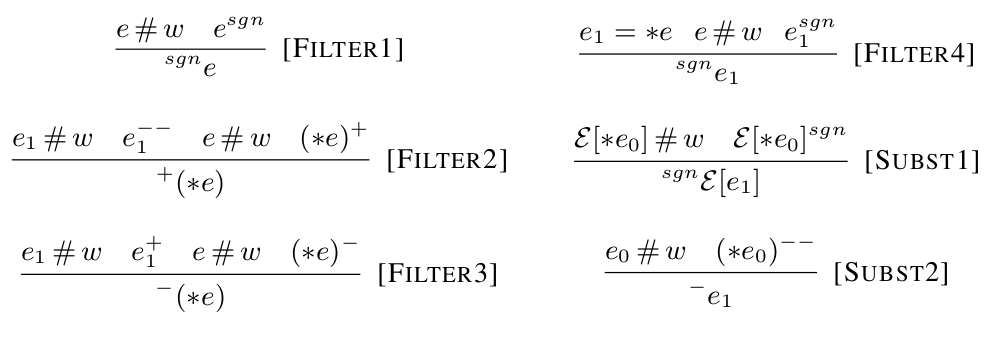
\includegraphics[width=1.0\columnwidth]{figs/rules_assignment}
   \caption{Deduction rules for the analysis on assignments.}
   \label{fig:rule_ass}
\end{figure}

where $S'=S\cup pt(e_0)$, and $H',M'$ are derived using the deduction rules 
described in Figure~\ref{fig:rule_ass}, where $e^+$ and $e^-$ represent 
respectively $e\in H$ and $e\in M$ (hit/miss expressions in the post-state); 
$^+e$ and $^-e$ for $e\in H'$ and $e\in M'$ (hit/miss expressions in the 
pre-state); and $e^{--}$ denotes that $Miss(e,(S,H,M))$. The set $\omega$ is 
the set of regions potentially written by the assignment: $w=pt(e_0)$. Hence,
an expression has the same value before and after the statement if it is 
disjoint from $\omega$. 
[FILTER 1-4] judge which expressions are reserved from the post-state to the 
pre-state. [SUBST 1-2] generate new elements in the Hit and Miss sets.


\subsubparagraph{(2) Allocations}

\[
\Vert *e_0 \gets malloc \Vert(d)=\begin{cases}
\bot& \text{if $UnaliasedHit \wedge (*e_0 \in H \wedge e_0\#\omega)$},\\
\Vert *e_0 \gets 0 \Vert (d)& 
  \text{if $UnaliasedHit \vee (Miss(*e_0,d) \wedge e_0\#\omega)$},\\
\top& \text{otherwise}.
\end{cases}
\]

where $d=(S,H,M)$, $\omega=pt(e_0)$, and 
$UnaliasedHit=\exists(*e)\in H:pt(e)\cap\omega =\emptyset$.
It denotes that there is some expression unaliased to $*e_0$ also 
references the cell. Thus, if it holds as well as $(*e_0)^+$, a contradiction
occurs. Or, if there is evidence that the error cell has not been 
allocated at this site, it proceeds past this statement, treating the 
allocation as a nullification $*e_0 \gets 0$.

\subsubparagraph{(3) Deallocations}

\[
\Vert free(*e_0) \Vert(S,H,M)=\begin{cases}
\bot& \text{if $e \in H$},\\
(S,H,M)& \text{if $(Miss(e,(S,H,M))$},\\
(S,H,M\cup {e})& \text{otherwise}.
\end{cases}
\]

A contradiction occurs if the reference lost is a reference to a cell that has 
already been freed, which is actually not an error. Otherwise, the analysis 
knows that $e$ misses in the pre-state.

\subsubparagraph{(4) Conditions}

\[
\Vert cond(e_0\equiv e_1)\Vert(S,H,M)=\begin{cases}
\bot& \text{if $Infeasible(S,H",M")$},\\
Cleanup(S,H",M")& \text{otherwise}.
\end{cases}
\]

\begin{figure}
  \centering
  
\includegraphics[width=1.0\columnwidth]{figs/rules_cond}
   \caption{Deduction rules for the analysis on conditions.}
   \label{fig:rule_cond}
\end{figure}

where $H"=H\cup H'$, $M"=M\cup M'$, $H'$ and $M'$ are the new hit and miss 
expressions derived using the deduction rules in Figure~\ref{fig:rule_cond}. 
The conditions can help derive new hit and miss expressions in the pre-state 
because they infer that the (in)equality is succeeded in the post-state.
